\chapter{Analisis}
\label{chap:analisis}

Pada bab ini dijelaskan mengenai hasil analisis yang dilakukan untuk penelitian ini, yaitu analisis mengenai leksikon, proses morphological parsing, morfotaktik, use case dan skenario dari perangkat lunak, dan yang terakhir diagram kelas dari perangkat lunak yang akan dibangun.

%\section{Analisis Perangkat Lunak Serupa}
%\label{sec:mpYangSudahAda}
%
%Pada tahun 2008, Pisceldo dkk pernah membuat sebuah artikel yang berjudul "A Two-Level Morphological Analyser for the Indonesian Language"\cite{manurung:08:indonesian}. Artikel ini berisi tentang usaha pembuatan perangkat lunak \textit{morphological analyser} untuk bahasa Indonesia melalui pendekatan \textit{two-level}. Perangkat lunak ini dapat memproses kata yang merupakan hasil afiksasi dan reduplikasi. 
%
%Proses morphological analysis mengambil informasi berupa kategori gramatikal dari sebuah kata berdasarkan aturan morfologi yang ada. Pada penelitian ini dipakai \textit{two-level morphology approach}, prosesnya dipecah menjadi menentukan aturan morfotaktik dan morfofonemik. Aturan ini dimodelkan ke dalam network \textit{finite-state transducers} dan diimplementasikan dengan \textbf{xfst} dan \textbf{lexc}. Sistem yang dihasilkan dari penelitian ini bisa menangani reduplikasi, proses morfologi yang tidak memerlukan penggabungan kata (non-concatenative).
%
%\subsection{Desain}
%\label{sec:desainMPYangSudahAda}
%
%Desain perangkat lunak dibagi dalam dua komponen:
%	\begin{itemize}
%		\item Morfotaktik: menentukan kelas morfem mana yang bisa mengikuti kelas morfem lain dalam sebuah kata
%		\item Morfofonemik: memodelkan perubahan fonologi yang terjadi pada proses pembentukan kata
%	\end{itemize}
%
%Adapun desain leksikon yang digunakan terdiri dari 4 kelas yaitu verbs, nouns, adjectives, dan 'etc' (pronouns, adverbs, numbers, dan particles)
%
%Desain tag yang digunakan:
%	\begin{itemize}
%		\item Normal tags: $+VERB, +NOUN, +ADJ, +BAREVERB, +BARENOUN, +BAREADJ, \\+BAREETC, +AV, +PASS, +UV,$ dan $+REDUP$
%		\item Special tags: $+CAUS\_KAN, +APPL\_KAN, +CAUS\_I, +APPL\_I, +ACTOR, \\+INSTRUMENT$
%	\end{itemize}
%	
%Detailnya adalah sebagai berikut:
%	\begin{itemize}
%		\item Tag seperti $+VERB, +NOUN$, dan $+ADJ$ menandai kata yang sudah melalui proses morfologi
%		\item Tag seperti $+BAREVERB, +BARENOUN, +BAREADJ,$ dan $+BAREETC$ menandai kata dasar
%		\item Tag seperti $+AV, +PASS,$ dan $+UV$ menandai kategori gramatikal, $+AV$ untuk active voice, $+PASS$ untuk passive voice, dan $+UV$ untuk undergoer voice
%		\item Tag $+REDUP$ untuk menandai reduplikasi
%		\item Tag $+CAUS\_KAN, +APPL\_KAN, +CAUS\_I$, dan $+APPL\_I$ menandai kata tersebut merupakan causative atau applicative dengan melihat akhirannya
%		\item Tag $+ACTOR$ dan $+INSTRUMENT$ menandai kata tersebut membawa makna actor atau instrument
%	\end{itemize}
%	
%Aturan morfotaktik untuk bahasa Indonesia ada 13 aturan, 10 aturan untuk pembubuhan afiks (meN-, peN-, di-, per-, ber-, ter-, ke-, -an, -kan, dan -i), dan 3 aturan untuk reduplikasi (utuh, sebagian, berimbuhan).
%
%Contoh aturan morfotaktik pembubuhan afiks:
%	\begin{itemize}
%		\item membersihkan (meN+bersih+kan). Kata bersih adalah adjective, setelah digabung dengan meN-kan hasilnya adalah verb.
%		\item pembelajaran (peN+ber+ajar+an). Kata ajar adalah verb, setelah digabung dengan peN-ber-an, hasilnya adalah noun.
%		\item keberhasilan (ke+ber+hasil+an). Kata hasil adalah noun, setelah digabung dengan ke-ber-an, hasilnya tetap noun.
%		\item terangi (terang+i). Kata terang adalah adjective, setelah digabung dengan -i, hasilnya adalah verb.
%	\end{itemize}
%
%Contoh aturan morfotaktik reduplikasi:
%	\begin{itemize}
%\item buku-buku. Kata buku-buku, adalah noun, dihasilkan dari kata buku, yang juga adalah sebuah noun.
%\item kekayaan-kekayaan (reduplikasi dari ke+kaya+an). Kata kaya adalah adjective. Setelah mengalami proses morfologi, hasilnya adalah noun.
%\item berlari-lari (ber+lari-lari). Kata lari adalah verb. Setelah mengalami proses morfologi, hasilnya adalah juga verb.
%\item tanam-menanam (tanam-meN+tanam). Kata tanam adalah verb. Setelah mengalami proses morfologi, hasilnya adalah juga verb.
%	\end{itemize}
%
%Selama tahap penerapan aturan morfotaktik, ada beberapa langkah yang harus dilakukan, yaitu penambahan prefiks dan preprefiks, penambahan stems dan part-of-speech, penambahan sufiks, dan proses akhir berupa penambahan tags.
%
%Aturan morfofonemik untuk bahasa Indonesia dibagi dalam dua kelompok, ada 4 aturan untuk memodelkan perubahan pada kata dasar dan ada 7 aturan untuk memodelkan perubahan pada afiks.
%
%Aturan pada perubahan kata dasar:
%	\begin{itemize}
%		\item Mengganti /k/ menjadi /ng/ jika mendapat awalan meN- atau peN-.
%Contoh: meN+kantuk menjadi mengantuk.
%		\item Mengganti /s/ menjadi /ny/ jika mendapat awalan meN- atau peN-.
%Contoh: peN+sebaran menjadi penyebaran.
%		\item Mengganti /p/ menjadi /m/ jika mendapat awalan meN- atau peN-.
%Contoh: peN+pakai menjadi pemakai.
%		\item Mengganti /t/ menjadi /n/ jika mendapat awalan meN- atau peN-.
%Contoh: meN+tertawakan menjadi menertawakan.
%	\end{itemize}
%
%Aturan pada perubahan afiks:
%	\begin{itemize}
%		\item Penghapusan /N/ jika awalan meN- diikuti /l/, /m/, /n/, /r/, /y/, /w/, /t/, /s/, /p/, /k/ atau jika awalan peN diikuti /l/, /m/, /n/, /r/, /d/, /w/, /t/, /s/, /p/, /k/. 
%Contoh: meN+lukis menjadi melukis.
%		\item Penghapusan /r/ jika awalan ber-, ter-, atau per- diikuti oleh /r/ atau kata yang suku pertamanya berakhir dengan /er/. 
%Contoh: ber+runding menjadi berunding.
%		\item Penggantian /N/ dengan /n/ jika meN- diikuti oleh /d/, /c/, /j/, /sy/ atau jika peN- diikuti /d/, /c/, /j/. 
%Contoh: peN+jual menjadi penjual.
%		\item Penggantian /N/ dengan /m/ jika meN- atau peN- diikuti oleh /b/, /f/. 
%Contoh: peN+buru menjadi pemburu.
%		\item Penggantian /N/ dengan /nge/ jika meN- diikuti oleh kata dengan satu suku. 
%Contoh: meN+rem menjadi mengerem.
%		\item Penggantian /N/ dengan /l/ jika peN- diikuti dengan kata ajar. 
%Contoh: peN+ajar menjadi pelajar.
%		\item Penggantian /r/ dengan /l/ jika ber- diikuti dengan kata ajar. 
%Contoh: ber+ajar menjadi belajar.
%	\end{itemize}
%
%Desain dari aturan morfofonemik untuk reduplikasi secara umum sama dengan afiksasi karena proses morfofonemik pada reduplikasi terjadi saat proses afiksasi dilakukan.
%
%Pada kasus di mana perubahan terjadi pada afiks dan kata dasar sekaligus, perlu ada beberapa penyesuaian aturan untuk digunakan pada bentuk reduplikasi. Contoh pada aturan morfofonemik penggantian /k/ menjadi /ng/ dan penghapusan /N/ yang bekerja bersamaan, awalnya adalah penghapusan /k/ dan penggantian /N/ dengan /ng/. Namun, pendekatan ini tidak bekerja jika melibatkan reduplikasi. Kata mengotak-ngotakkan tidak akan dianalisis dengan tepat jika morphological analyser menggunakan aturan penghapusan /k/ dan penggantian /N/ dengan /ng/. Kata mengotak-ngotakkan dihasilkan dari kata dasar kotak yang dimodifikasi dengan reduplikasi berafiks meN-kan. Jika penghapusan /k/ dan penggantian /N/ dengan /ng/ digunakan, hasil dari proses tersebut adalah kata mengotak-otakkan yang mana tidak valid. Ini adalah alasan dalam reduplikasi aturannya diubah menjadi penggantian /k/ menjadi /ng/ dan penghapusan /N/ sehingga dihasilkan kata mengotak-ngotakkan.
%
%\subsection{Implementasi}
%\label{sec:implementasiMPYangSudahAda}
%
%Morphological analyser bahasa Indonesia ini diimplementasikan menggunakan \textbf{xfst} and \textbf{lexc}. Aturan morfotaktik diimplementasikan dengan \textbf{xfst} sementara aturan morfofonemik diimplementasikan dengan \textbf{lexc}.
%
%Implementasi aturan morfotaktik dapat diilustrasikan dengan \textit{finite-state automata} yang ditunjukkan pada gambar \ref{gambar-fsa-morfotaktik-contoh}. Kata bahasa Indonesia yang valid, yaitu yang dihasilkan melalui proses morfologi yang benar, dapat diterima oleh automata, sementara yang tidak valid ditolak.
%
%Berawal dari root, setiap state menentukan kemungkinan lanjutan state selagi mengambil simbol tertentu. Dalam \textbf{lexc}, state ini disebut \textit{continuation classes}. Semua continuation classes yang bisa dicapai dari root menampilkan prefiks dan preprefiks. Perbedaan di antara keduanya diperlukan untuk mengenali variasi morfologi berupa adanya 2 prefiks, seperti prefiks memper-, diper-. Dari sana, continuation class selanjutnya adalah stem, di mana kata dasar diambil. Ini diteruskan dengan beberapa classes yang menampilkan kemungkinan sufiks, namun ada juga class Redup1 dan Redup2 yang muncul sebelum dan setelah sufiks. Fungsinya adalah untuk menangani reduplikasi. Terakhir, tagEmit class memproses semua tags yang belum ditangani oleh class sebelumnya.
%
%\begin{figure}[H]
%\centering
%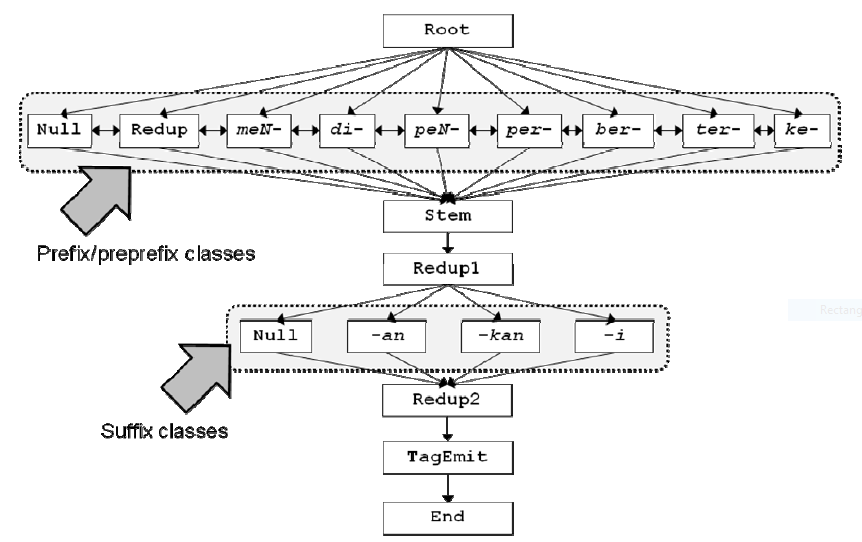
\includegraphics[scale=0.5]{Gambar/gambar-fsa-morfotaktik-contoh}
%\caption[Ilustrasi proses morfotaktik]{Ilustrasi proses morfotaktik\cite{manurung:08:indonesian}} 
%\label{gambar-fsa-morfotaktik-contoh}
%\end{figure}
%
%%Selama proses morfotaktik ini, kita menggunakan flag diacritics, fitur penting dari \textbf{lexc} yang memperkirakan kemampuan dari struktur fitur, di antaranya mampu menentukan hambatan tertentu untuk memastikan hanya jalur yang valid dari network yang dilewati. Satu keuntungan dari pendekatan ini adalah perbaikan dari representasi network yang ringkas. Ada 3 flag diacritics yang digunakan dalam model kita: positive setting (@P.feat.val@), required test (@R.feat.val@), dan disallow test (@D.feat.val@). Dengan menggunakan diacritics ini, kita dapat menetapkan nilai dan hambatan dari aspek tertentu, yang harus konsisten sepanjang jalur.
%
%%Sebagai contoh, prefiks meN- bisa dikombinasikan dengan sufiks -kan dan -i, tapi tidak -an. Kita dapat menampilkan ini dengan fitur, misal PREF, yang dipasangkan pada meN pada (pre)prefix state (@P.PREF.meN@). Tes yang cocok selanjutnya ditambahkan pada suffix states, misal jalur saat ini melewati prefix state meN-, @R.PREF.meN@ menetapkan ada sufiks yang harus dipasangkan, sementara @D.PREF.meN@ mencegah sufiks diterapkan.
%
%Sudah dibahas di atas bahwa morfologi bahasa Indonesia mengandung proses reduplikasi. Sangat sulit menangani ini dengan regular grammar yang diimplementasikan dengan finite-state automata. Oleh karena itu, digunakan fitur compile-replace dalam \textbf{xfst}. Fitur ini memperbolehkan pengulangan bahasa yang kompleks dengan menggunakan tanda $"^{\wedge}["$ dan $"^{\wedge}]"$ untuk menandai bagian reduplikasi. Tanda kurung siku kanan juga ditambah dengan $^{\wedge}2$ untuk menandakan duplikasi; sehingga lengkapnya adalah $"^{\wedge}["$ dan $"^{\wedge}2^{\wedge}]"$. Dengan definisi network ini, \textbf{xfst} melakukan compiles dan post-processes dari keterangan ini untuk menghasilkan network baru yang bisa mengenali reduplikasi. Contoh, $"^{\wedge}[buku^{\wedge}2^{\wedge}]"$ akan dicompile menjadi bukubuku.
%
%Idenya adalah untuk memasukkan $"^{\wedge}["$ dan $"^{\wedge}2^{\wedge}]"$ pada posisi yang tepat. Karena banyaknya tipe reduplikasi dalam bahasa Indonesia, aturan reduplikasi dapat ditemukan pada state Redup (pre)prefix dan state Redup1 dan Redup2. State prefix Redup mengambil tanda kurung siku $"^{\wedge}["$ dan mengeset flag yang tepat sebagai pengingat bahwa tanda kurung siku kanan dibutuhkan. State Redup1 bertanggung jawab untuk menutup reduplikasi sebagian dan reduplikasi berafiks, contoh di mana sufiks tidak diikutkan dalam reduplikasi, sementara state Redup2 bertanggung jawab untuk menutup reduplikasi utuh, contoh di mana sufiks menjadi bagian dari proses reduplikasi. Baik state Redup1 dan Redup2 mengecek nilai dari flag REDUP yang diset pada prefix state Redup.
%
%Transducer yang utuh terdiri dari aturan morfotaktik dan morfofonemik sehingga keluaran dari implementasi aturan morfotaktik menjadi masukan bagi implementasi aturan morfofonemik. Dari contoh sebelumnya, keluaran dari implementasi aturan morfotaktik adalah me$^{\wedge}$Npukuli dan menjadi masukan bagi implementasi aturan morfofonemik.
%
%Berbeda dengan implementasi aturan morfotaktik yang bisa direpresentasikan dengan diagram alur proses, implementasi dari aturan morfofonemik berisi aturan-aturan perubahan dan penggantian fonem seperti yang sudah dipaparkan sebelumnya. Pada gambar \ref{gambar-implementasi-aturan-morfofonemik} berikut adalah contoh implementasi dari aturan 'RG4' yang mengkodekan penghapusan /N/ dan penggantian 4 jenis fonem pada kata dasar:
%
%\begin{figure}[H]
%\centering
%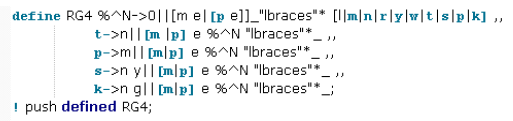
\includegraphics[scale=0.6]{Gambar/gambar-implementasi-aturan-morfofonemik}
%\caption[Implementasi aturan morfofonemik]{Implementasi aturan morfofonemik\cite{manurung:08:indonesian}} 
%\label{gambar-implementasi-aturan-morfofonemik}
%\end{figure}
%
%Aturan ini terdiri dari 5 aturan yang bekerja secara paralel. Aturan pertama adalah penghapusan /N/ pada prefiks jika /me/ atau /pe/ diikuti oleh kata dasar dengan fonem awal /l/, /m/, /n/, /r/, /y/, /w/, /t/, /s/, /p/, atau /k/.
%
%Aturan selanjutnya terdiri dari 4 aturan perubahan fonem awal pada kata dasar yang diberikan prefiks /me$^{\wedge}$N/ atau /pe$^{\wedge}$N/, dan fonem awal pada kata dasarnya adalah /t/, /p/, /s/, atau /k/. Lebih detail, fonem /t/ akan diganti dengan /n/, fonem /p/ diganti dengan /m/, fonem /s/ diganti dengan /ny/, dan fonem /k/ diganti dengan /ng/.
%
%Contoh masukan me$^{\wedge}$Npukuli pada proses sebelumnya memenuhi aturan penghapusan /N/ dan penggantian fonem awal /p/ dari kata dasar dengan fonem /m/. Kata me$^{\wedge}$Npukuli akan diproses menjadi kata memukuli. Kata tersebut merupakan kata yang valid dalam bahasa Indonesia dan proses berakhir di sini.
%
%Pengujian dilakukan dengan menjalankan tes kasus dengan kata yang diambil dari Kamus Besar Bahasa Indonesia versi elektronik. Pengujian dilakukan pada implementasi dari aturan morfotaktik dan morfofonemik secara terpisah. Untuk menguji kemampuan dari analyser untuk menerima masukan yang valid dan tidak valid, tes kasus yang digunakan mengandung penulisan kombinasi morfem yang valid dan tidak valid. Hasil dari pengujian ditampilkan pada tabel \ref{tabel-hasil-pengujian-morfotaktik}, yang menunjukkan hasil pengujian morfotaktik, dan tabel \ref{tabel-hasil-pengujian-morfofonemik}, yang menunjukkan hasil pengujian morfofonemik. Kolom Analisis menampilkan hasil dari sistem yang memproses penguraian struktur morfologi dari kata dalam bahasa Indonesia. Contoh, diberikan masukan kata memukul, sistem diharapkan menghasilkan keluaran pukul+Verb+AV. Sementara, kolom Sintesis menangani situasi yang sebaliknya, di mana masukannya adalah tag morfologi dan sistem diharapkan menghasilkan keluaran berupa kata yang valid dalam bahasa Indonesia.
%
%\begin{table}[H]
%\centering
%\begin{tabular}{|c|c|c|c|}
%\hline
%\textbf{Hasil} & \textbf{Analisis} & \textbf{Sintesis} & \textbf{Jumlah} \\
%\hline
%1. Hasil benar & 103 & 43 & 146 \\
%\hline
%2. Beberapa hasil, ada yang benar & 46 & 106 & 152 \\
%\hline
%3. Hasil salah & 3 & 3 & 6 \\
%\hline
%\textbf{Jumlah} & 152 & 152 & 308 \\
%\hline
%\end{tabular}
%\caption{Hasil pengujian morfotaktik\cite{manurung:08:indonesian}}
%\label{tabel-hasil-pengujian-morfotaktik}
%\end{table}
%
%\begin{table}[H]
%\centering
%\begin{tabular}{|c|c|c|c|}
%\hline
%\textbf{Hasil} & \textbf{Analisis} & \textbf{Sintesis} & \textbf{Jumlah} \\
%\hline
%1. Hasil benar & 51 & 21 & 72 \\
%\hline
%2. Beberapa hasil, ada yang benar & 6 & 36 & 42 \\
%\hline
%3. Hasil salah & 1 & 1 & 2 \\
%\hline
%\textbf{Jumlah} & 58 & 58 & 116 \\
%\hline
%\end{tabular}
%\caption{Hasil pengujian morfofonemik\cite{manurung:08:indonesian}}
%\label{tabel-hasil-pengujian-morfofonemik}
%\end{table}
%
%Ada tiga kategori hasil pengujian, kategori pertama adalah ketika sistem menghasilkan sebuah hasil analisis atau sintesis yang benar atau tidak menghasilkan apapun untuk tes kasus yang tidak valid. Kategori kedua adalah ketika sistem diberikan masukan valid dan menghasilkan beberapa jawaban, yang salah satunya adalah jawaban yang diharapkan. Terakhir, kategori ketiga adalah ketika sistem gagal menganalisis atau menyintesis tes kasus yang valid atau tidak memproduksi jawaban yang tepat ketika diberikan tes kasus yang tidak valid.
%
%Dari tabel, dapat dilihat bahwa hasil untuk proses analisis lebih baik dari proses sintesis, di mana sistem cenderung memproduksi lebih dari satu kemungkinan jawaban. Contoh, sistem ini mampu menghasilkan kata memukul pada proses analisis, namun ketika proses sintesis untuk pukul+Verb+AV, sistem menghasilkan beberapa kemungkinan jawaban yaitu memukulkan, memperpukuli, mengepukulkan, dll. Ini menandakan diperlukan tag yang lebih baik untuk fitur morfologi.

\section{Leksikon}
\label{sec:leksikon}
Leksikon, seperti ditulis pada subbab \ref{sec:morfemDasarDLL}, dapat dipadankan dengan istilah \textit{kosakata} atau \textit{perbendaharaan kata}. Leksikon dibutuhkan pada proses \textit{morphological parsing} untuk mengetahui apakah sebuah kata yang sedang diproses adalah sebuah kata dasar yang valid atau tidak dalam bahasa Indonesia. Leksikon menyimpan kumpulan kata dasar dan turunannya untuk nantinya diakses ketika proses \textit{morphological parsing} dilakukan. Kata turunan adalah kata yang merupakan hasil dari proses morfologi berupa afiksasi, reduplikasi, dan komposisi dari kata dasar yang bersangkutan.

Leksikon dalam proses \textit{morphological parsing} harus bisa diakses dengan cepat dan efektif. Hal ini dikarenakan leksikon akan diakses sangat sering dalam proses ini. Leksikon akan diakses sekitar 3-5 kali untuk setiap kata yang sedang diproses. Oleh karena itu, leksikon perlu disimpan pada struktur data yang memungkinkan waktu akses yang cepat supaya keseluruhan proses dapat dijalankan dalam waktu yang masuk akal. 

Struktur data yang saat ini terkenal paling cepat untuk diakses adalah struktur data \textit{trie}. Trie adalah struktur data berbentuk pohon yang menyimpan himpunan string yang jika ditelusuri setiap node mulai dari akar hingga daun akan membentuk suatu string yang merupakan kunci yang kita cari. Setiap string yang dihasilkan dari node awal yang sama akan mempunyai awalan (prefiks) yang sama, karena itulah trie disebut juga pohon prefiks.

\begin{figure}[H]
\centering
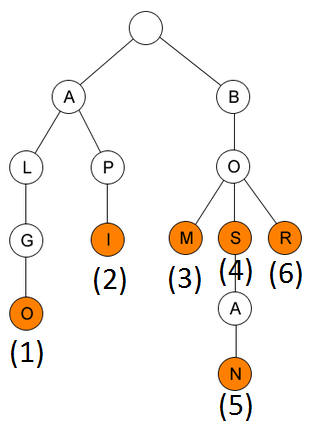
\includegraphics[scale=0.75]{Gambar/gambar-trie}
\caption[Struktur data trie]{Struktur data trie} 
\label{bagan-trie}
\end{figure}

Struktur data trie yang digambarkan pada bagan \ref{bagan-trie} menyimpan enam string kunci dari dua buah awalan, yaitu string "A" dan "B". Jika kita telusuri dari node akar "A" sampai node daun "O", kita akan mendapat string "ALGO" yang ditandai dengan nomor (1). String lain yang disimpan pada contoh tersebut adalah string "API" pada nomor (2), string "BOM" pada nomor (3), string "BOS" pada nomor (4), string "BOSAN" pada nomor (5), dan string "BOR" pada nomor (6).

Perlu diperhatikan bahwa sebuah string kunci tidak harus disimpan dengan node terakhir ada pada posisi daun, seperti pada string "BOS" pada nomor 4. Node terakhir pada string tersebut merupakan node internal. Penyimpanan seperti ini bisa dilakukan dengan menandai setiap node yang merupakan akhir dari sebuah string yang membentuk kata.

Ada dua jenis kata yang disimpan dalam leksikon, yaitu kata dasar dan kata turunan. Contoh kata dasar adalah kata 'sapu', 'makan', dan 'kerja' sementara contoh kata turunan adalah kata 'menyapu', 'makan-makan', dan 'kerja bakti'. Kata-kata turunan ini adalah kata yang merupakan hasil dari proses morfologi berupa afiksasi, reduplikasi, atau komposisi. Kata turunan disimpan sebagai bagian dari kata dasar dan dapat diakses ketika dibutuhkan. 

Dalam Kamus Besar Bahasa Indonesia, ada beberapa kata yang merupakan hasil dari proses morfologi yang sudah diserap dan dianggap sebagai sebuah kata dasar. Contohnya adalah kata 'gerigi' yang merupakan hasil penyisipan infiks -er- pada kata 'gigi', kata 'abu-abu' yang merupakan hasil reduplikasi dari kata 'abu', dan kata 'rumah sakit' yang merupakan hasil komposisi dari kata 'rumah' dan kata 'sakit'. Dalam kasus tersebut, untuk kata yang merupakan hasil penyisipan infiks akan disimpan sebagai sebuah kata dasar dalam leksikon sementara untuk kata yang merupakan hasil reduplikasi dan komposisi akan disimpan sebagai kata turunan dari kata dasar yang bersangkutan.

Untuk kata turunan yang merupakan hasil afiksasi berupa pengimbuhan klitika, kata tersebut tidak disimpan sebagai bentuk turunan dalam leksikon karena dianggap terlalu produktif. Contohnya adalah kata 'bukumu' tidak disimpan sebagai bentuk turunan dari kata 'buku' dan kata 'mobilnya' tidak disimpan sebagai bentuk turunan dari kata 'mobil'. Sementara ada kasus di mana klitika \textit{-nya} merupakan bagian dari konfiks \textit{se-nya}, di mana konfiks adalah gabungan antara prefiks dan sufiks yang diimbuhkan secara bersamaan. Timbul kerancuan apakah \textit{-nya} di sini akan dianggap sebagai klitika atau sufiks. Untuk penelitian kali ini, bentuk \textit{-nya} akan dianggap sebagai klitika karena \textit{-nya} sebagai klitika dianggap lebih produktif daripada sebagai sufiks dalam kesatuan konfiks \textit{se-nya}.

Dalam Kamus Besar Bahasa Indonesia Dalam Jaringan (KBBI daring)\footnote{https://kbbi.kemdikbud.go.id/}, kata dasar dan kata turunan disimpan secara terpisah namun keduanya dapat dicari melalui kolom pencarian. Sementara pada Kamus Besar Bahasa Indonesia Luar Jaringan (KBBI luring)\footnote{http://ebsoft.web.id/kbbi-kamus-besar-bahasa-indonesia-offline-gratis/}, hanya kata dasar saja yang bisa dicari melalui kolom pencarian namun semua kata turunannya juga disimpan sebagai bagian dari sebuah kata dasar. Pada penelitian kali ini akan digunakan struktur penyimpanan dan pencarian seperti pada KBBI luring.

Struktur penyimpanan seperti pada KBBI luring memungkinkan untuk mengenali perbedaan antara kata dasar dan kata yang telah melalui proses morfologi seperti afiksasi, reduplikasi, dan komposisi. Perangkat lunak yang dirancang pada penelitian ini harus dapat menentukan apakah sebuah kata merupakan kata dasar yang valid atau tidak dalam bahasa Indonesia. Pencarian kata dasar dalam leksikon harus dapat melakukan hal tersebut sehingga pencarian hanya bisa dilakukan terhadap kata dasar saja dan tidak dengan kata turunannya. Kata turunan perlu disimpan dalam leksikon untuk melakukan validasi terhadap hasil dari proses parsing yang dilakukan oleh perangkat lunak. %Kata yang telah melalui proses parsing dicek kebenarannya apakah merupakan kata turunan yang valid atau tidak dari kata dasar yang bersangkutan.


\section{Proses \textit{Morphological Parsing}}
\label{sec:morphologicalParsing}

Pada subbab \ref{sec:prosesMorfologi} telah dibahas mengenai proses morfologi, yang pada dasarnya adalah proses pembentukan kata melalui beberapa proses, yaitu pembubuhan afiks (afiksasi), pengulangan (reduplikasi), dan penggabungan (komposisi). Proses \textit{morphological parsing} merupakan kebalikan dari proses morfologi. Masukan bagi proses \textit{morphological parsing} adalah kata atau kalimat yang telah melalui proses morfologi dan keluarannya adalah komponen-komponen penyusunnya.

Proses \textit{morphological parsing} untuk setiap kata dalam masukan dapat dituliskan sebagai berikut:
\begin{enumerate}
	\item Periksa leksikon, jika kata tersebut ada dalam leksikon, masukkan sebagai salah satu kemungkinan keluaran
	\item Periksa adanya kemungkinan afiks, baik itu prefiks, sufiks, maupun konfiks. Pisahkan afiks yang ditemukan dengan komponen kata yang lain dan lakukan proses parsing pada komponen kata tersebut
	\item Periksa adanya simbol penghubung (-), yang menandakan hasil proses reduplikasi, lalu lakukan proses parsing terhadap bentuk dasar dari kata tersebut
	\item Jika ada kata yang mengikuti, periksa kemungkinan kata yang sedang diproses dan kata yang mengikuti adalah dua kata hasil komposisi dengan melakukan pengecekan terhadap bentuk dasar dari kata tersebut
	%\item Jika sudah dilakukan pemisahan terhadap kemungkinan afiks namun kata yang sedang diproses tidak ditemukan dalam leksikon, kemungkinan kata tersebut bukan kata dalam bahasa Indonesia
\end{enumerate}

Leksikon yang dibuat dalam perangkat lunak ini juga menyimpan kata turunan yang valid dari setiap kata dasar yang ada. Setelah proses parsing selesai dilakukan, leksikon dapat melakukan validasi apakah kata turunan yang sudah diproses benar merupakan kata turunan yang valid dari kata dasar yang bersangkutan. 

Sebagai contoh, jika dilakukan proses \textit{morphological parsing} pada kata 'kemerah-merahan', maka prosesnya adalah sebagai berikut:
\begin{itemize}
	\item Periksa leksikon, kata tersebut tidak ditemukan dalam leksikon
	\item Periksa kemungkinan afiks, ditemukan kemungkinan konfiks $\lbrace$ke-an$\rbrace$ dan klofiks $\lbrace$ke-an$\rbrace$, lakukan proses parsing terhadap kata 'merah-merah'
	\item Ditemukan simbol penghubung (-) sehingga diketahui kata tersebut adalah hasil proses reduplikasi. Pisahkan kata dan lakukan proses parsing sehingga didapat hasilnya adalah reduplikasi dari kata dasar 'merah'
	\item Didapat dua kemungkinan hasil, yaitu reduplikasi kata 'merah' diikuti konfiksasi $\lbrace$ke-an$\rbrace$ dan reduplikasi kata 'merah' diikuti klofiksasi $\lbrace$ke-an$\rbrace$
	\item Lakukan validasi pada leksikon, dan didapatkan kata turunan yang valid adalah reduplikasi kata 'merah' diikuti konfiksasi $\lbrace$ke-an$\rbrace$
	\item Hasil akhir proses parsing adalah bentuk dasar $\lbrace$merah$\rbrace$ + reduplikasi + konfiks $\lbrace$ke-an$\rbrace$
\end{itemize}

%Perlu diperhatikan, jika sebuah kata merupakan hasil proses reduplikasi, maka kata tersebut tidak mungkin adalah hasil proses komposisi, demikian juga sebaliknya.

Untuk kata dengan kemungkinan hasil parsing lebih dari satu, seperti kata 'beruang', prosesnya adalah sebagai berikut:
\begin{itemize}
	\item Periksa leksikon, ditemukan bentuk dasar $\lbrace$beruang$\rbrace$, masukkan sebagai salah satu kemungkinan keluaran
	\item Periksa kemungkinan afiks pada kata 'beruang'
	\item Didapatkan prefiks $\lbrace$ber-$\rbrace$ + bentuk dasar $\lbrace$uang$\rbrace$, masukkan sebagai salah satu kemungkinan keluaran
	\item Periksa kemungkinan adanya fonem yang dilesapkan pada bentuk dasar, yaitu fonem 'r', dan didapatkan prefiks $\lbrace$ber-$\rbrace$ + bentuk dasar $\lbrace$ruang$\rbrace$, masukkan sebagai salah satu kemungkinan keluaran
	\item Lakukan validasi pada leksikon terhadap kata turunan dari bentuk dasar $\lbrace$uang$\rbrace$ dan $\lbrace$ruang$\rbrace$
	\item Hasil akhir proses parsing adalah bentuk dasar $\lbrace$beruang$\rbrace$, prefiks $\lbrace$ber-$\rbrace$ + bentuk dasar $\lbrace$uang$\rbrace$, dan prefiks $\lbrace$ber-$\rbrace$ + bentuk dasar $\lbrace$ruang$\rbrace$
\end{itemize}

Bentuk-bentuk yang tidak secara khusus ada dalam bahasa Indonesia seperti angka, nama orang, dan kata dalam bahasa asing ditulis sebagai \textit{bentuk asing} dalam keluaran dari proses parsing.

Beberapa contoh yang sudah dibahas di atas adalah contoh proses parsing yang dilakukan pada sebuah kata dalam bahasa Indonesia. Perangkat lunak \textit{morphological parser} yang dirancang pada penelitian ini akan dapat memproses tidak hanya kata tapi juga kalimat dan paragraf yang ditulis dalam bahasa Indonesia. Proses parsing pada kalimat dan paragraf memerlukan beberapa langkah tambahan yaitu:

\begin{enumerate}
	\item Hilangkan tanda baca yang tidak diperlukan dalam proses parsing. Tanda baca yang diperlukan dalam proses parsing hanya tanda baca penghubung kata (-) sebagai tanda hasil proses reduplikasi
	\item Gantikan tanda baca yang dihilangkan dengan karakter kosong ("")
	\item Pisahkan setiap kata berdasarkan karakter spasi yang memisahkan kata lalu lakukan proses parsing untuk setiap kata tersebut
\end{enumerate}


%\section{Pembentuk Kata}
%\label{sec:pembentukKata}
%
%Pada subbab \ref{sec:prosesMorfologi} yang membahas tentang proses morfologi, telah disinggung bahwa proses morfologi dalam bahasa Indonesia melibatkan dua komponen yaitu bentuk dasar dan alat pembentuk kata. Bentuk dasar adalah bentuk yang kepadanya dilakukan proses morfologi sedangkan alat pembentuk kata adalah komponen yang digunakan dalam proses morfologi yaitu afiks dalam proses afiksasi, pengulangan dalam proses reduplikasi, dan penggabungan dalam proses komposisi.
%
%Dalam proses afiksasi, sebuah afiks diimbuhkan kepada sebuah bentuk dasar sehingga menghasilkan sebuah kata baru yang merupakan hasil dari proses morfologi. Berdasarkan letak pengimbuhannya, afiks terdiri dari beberapa jenis, yaitu prefiks, infiks, sufiks, dan konfiks. Selain itu, dikenal pula afiks yang sekilas mirip dengan konfiks namun berbeda yang disebut klofiks. Lalu dalam pertuturan sering juga digunakan afiks yang disebut dengan klitika.
%
%Prefiks adalah afiks yang dibubuhkan di kiri bentuk dasar. Jenis-jenis prefiks adalah \textit{me-}, \textit{pe-}, \textit{per-}, \textit{di-}, \textit{ber-}, \textit{ter-}, \textit{se-}, dan \textit{ke-}. Lalu infiks adalah afiks yang dibubuhkan di tengah kata, biasanya pada suku awal kata. Jenis-jenis infiks adalah \textit{-el-}, \textit{-em-}, dan \textit{-er-}. Lalu sufiks adalah afiks yang dibubuhkan di kanan bentuk dasar. Jenis-jenis sufiks adalah \textit{-kan}, \textit{-an}, dan \textit{-i}. Perlu dicatat bahwa infiks sebagai alat pembentuk kata dalam bahasa Indonesia sudah tidak produktif pada saat ini.
%
%Konfiks adalah afiks yang dibubuhkan di kiri dan di kanan bentuk dasar secara bersamaan. Jenis-jenis konfiks adalah \textit{ke-an}, \textit{ber-an}, \textit{pe-an}, \textit{per-an}, dan \textit{se-nya}. Berbeda dengan konfiks, klofiks adalah dua atau tiga buah afiks yang dibubuhkan di kiri dan/atau di kanan bentuk dasar tetapi pembubuhannya tidak sekaligus, melainkan bertahap. Jenis-jenis klofiks adalah \textit{me-kan}, \textit{me-i}, \textit{memper-}, \textit{memper-kan}, \textit{memper-i}, \textit{ber-kan}, \textit{di-kan}, \textit{di-i}, \textit{diper-}, \textit{diper-kan}, \textit{diper-i}, \textit{ter-kan}, dan \textit{ter-i}.
%
%Klitika adalah adalah afiks yang dalam ucapan tidak mempunyai tekanan sendiri dan tidak merupakan kata karena tidak dapat berdiri sendiri. Berdasarkan letaknya, ada dua jenis klitika, yaitu proklitika dan enklitika. Proklitika adalah klitika yang dibubuhkan di kiri bentuk dasar sementara enklitika adalah klitika yang dibubuhkan di kanan bentuk dasar. Jenis-jenis proklitika adalah \textit{ku-} dan \textit{kau-} sementara jenis-jenis enklitika adalah \textit{-ku}, \textit{-mu}, \textit{-nya}, \textit{-lah}, \textit{-kah}, dan \textit{-pun}.
%
%Dalam proses reduplikasi, kata yang menjadi bentuk dasar dapat berupa sebuah kata dasar, seperti pada kata 'rumah-rumah' yang berasal dari kata dasar 'rumah'. Selain itu, bentuk dasar dapat pula berupa kata yang merupakan hasil dari proses afiksasi seperti pada kata 'berlari-lari' yang berasal dari kata 'berlari'. Proses reduplikasi juga dapat menghasilkan kata ulang yang antara kata pertama dan kata kedua tidak sama atau disebut dengan kata ulang berubah bunyi, seperti kata 'sayur-mayur' dan 'gerak-gerik'.
%
%Dalam proses komposisi, kata yang menjadi bentuk dasar dapat berupa sebuah kata dasar dan diikuti kata dasar lain yang tidak berhubungan dengan kata dasarnya dan hanya sebagai penjelas, seperti pada kata 'sate ayam' dan 'merah jambu'. Selain itu, dapat pula sebuah kata dasar diikuti oleh kata yang merupakan lawan kata atau antonimnya, seperti pada kata 'tua muda' dan 'jual beli'. Ada pula bentuk yang berupa sebuah kata dasar diikuti oleh kata yang tidak dapat berdiri sendiri dalam bahasa Indonesia, seperti pada kata 'gotong royong'.


\section{Morfotaktik}
\label{sec:morfotaktik}

Pada subbab \ref{sec:morfemDasarDLL} dan \ref{sec:morfemAfiks} telah dijelaskan mengenai morfem dasar dan morfem afiks. Morfem dasar adalah morfem yang dapat menjadi dasar dalam suatu proses morfologi. Sementara morfem afiks adalah morfem yang tidak dapat menjadi dasar dalam pembentukan kata, tetapi hanya menjadi unsur pembentuk dalam proses afiksasi. Kedua morfem tersebut dapat digabungkan dalam proses morfologi berupa proses afiksasi untuk membentuk sebuah kata. Proses penggabungan antara kedua morfem tersebut tidak boleh dilakukan secara sembarangan sehingga diperlukan aturan khusus yang mengatur penggabungan antara morfem dasar dan morfem afiks. Aturan ini disebut dengan morfotaktik. 

Morfem afiks terdiri dari prefiks, sufiks, dan konfiks. Jenis-jenis prefiks adalah prefiks \textit{ber-}, prefiks \textit{me-}, prefiks \textit{per-}, prefiks \textit{pe-}, prefiks \textit{di-}, prefiks \textit{ter-}, prefiks \textit{se-}, dan prefiks \textit{ke-}. Jenis-jenis sufiks adalah sufiks \textit{-kan}, sufiks \textit{-i}, dan sufiks \textit{-an}. Jenis-jenis konfiks adalah konfiks \textit{ke-an}, konfiks \textit{ber-an}, konfiks \textit{pe-an}, konfiks \textit{per-an}, dan konfiks \textit{se-nya}. Bahasa Indonesia membolehkan sebuah kata untuk dibentuk dengan dua buah prefiks, seperti contoh kata 'memperkuat' yang dibentuk dari kata dasar 'kuat' dengan dua buah prefiks, yaitu prefiks \textit{me-} dan prefiks \textit{per-}. Afiks yang diletakkan sebelum prefiks ini akan disebut dengan \textit{preprefiks}. 

Selain afiks yang sudah disebutkan, ada juga morfem afiks yang disebut dengan klitika. Berdasarkan letaknya, dibedakan adanya \textit{proklitika}, yaitu klitika yang berposisi di sebelah kiri kata yang diikuti dan \textit{enklitika} adalah klitika yang berposisi di belakang kata yang dilekati. Contoh proklitika adalah klitika \textit{ku-} dan \textit{kau-} dalam bentuk \textit{kubawa} dan \textit{kauambil}. Sementara contoh enklitika adalah klitika \textit{-ku}, \textit{-mu}, \textit{-nya}, dan \textit{-lah} pada bentuk \textit{bukuku}, \textit{nasibmu}, \textit{duduknya}, dan \textit{pergilah}. Secara pertuturan, klitika pada umumnya diletakkan di paling kiri atau di paling kanan dari sebuah kata, sehingga tidak mungkin ada morfem afiks atau morfem dasar lain yang diletakkan di sebelah kiri proklitika atau di sebelah kanan enklitika pada sebuah kata.

Aturan morfotaktik tidak hanya mengatur tentang proses penggabungan antara morfem dasar dengan morfem afiks, namun juga mengatur tentang proses pengulangan morfem dasar dalam proses reduplikasi dan proses penggabungan antara morfem dasar dengan morfem dasar lain dalam proses komposisi. Proses reduplikasi dan komposisi pun tidak boleh dilakukan secara sembarangan sehingga proses tersebut perlu juga diatur dalam aturan morfotaktik.

Aturan morfotaktik yang digunakan pada penelitian ini akan dijelaskan melalui tabel. Akan ada beberapa tabel untuk mewakili setiap jenis morfem, yaitu preprefiks, prefiks, akar, sufiks, dan konfiks. Setiap tabel akan menunjukkan komponen tersebut boleh didahului oleh komponen apa saja dan boleh diikuti oleh komponen apa saja. Komponen 'null' berarti boleh tidak didahului atau diikuti oleh komponen apapun. Berikut adalah tabel aturan morfotaktik untuk preprefiks, prefiks/konfiks, akar, dan sufiks/konfiks.

\begin{table}[H]
\centering
\begin{tabular}{|c|c|c|}
\hline
\textbf{Pendahulu} & \textbf{Preprefiks} & \textbf{Pengikut} \\
\hline
 proklitika&me-&per-\\
 null&di-&ke-\\
 & &ber-\\
 & &ter-\\
 \hline
 proklitika&pe-&ber-\\
 null& & \\
 \hline
 proklitika&ke-&ber-\\
 null& &pe-\\
 \hline
 proklitika&ber-&ke-\\
 null& &pe-\\
\hline
\end{tabular}
\caption{Tabel Aturan Morfotaktik untuk Preprefiks} 
\label{tabel-morfotaktik-preprefiks}
\end{table}

\begin{table}[H]
\centering
\begin{tabular}{|c|c|c|}
\hline
\textbf{Pendahulu} & \textbf{Prefiks/Konfiks} & \textbf{Pengikut} \\
\hline
 proklitika&per-&akar\\
 me-&ter-& \\
 di-& & \\
 null& & \\
 \hline
 proklitika&me-&akar\\
 null&di-& \\
  &se-& \\
 \hline
 proklitika&ke-&akar\\
 me-& & \\
 di-& & \\
 ber-& & \\
 null& & \\
 \hline
 proklitika&ber-&akar\\
 me-& & \\
 di-& & \\
 pe-& & \\
 ke-& & \\
 null& & \\
 \hline
 proklitika&pe-&akar\\
 ke-& & \\
 ber-& & \\
 null& & \\
\hline
\end{tabular}
\caption{Tabel Aturan Morfotaktik untuk Prefiks atau Konfiks} 
\label{tabel-morfotaktik-prefiks}
\end{table}

\begin{table}[H]
\centering
\begin{tabular}{|c|c|c|}
\hline
\textbf{Pendahulu} & \textbf{Akar} & \textbf{Pengikut} \\
\hline
 proklitika&akar&konfiks\\
 prefiks& &sufiks\\
 null& &reduplikasi\\
 & &komposisi\\
 & &enklitika\\
 & &null\\
\hline
\end{tabular}
\caption{Tabel Aturan Morfotaktik untuk Akar} 
\label{tabel-morfotaktik-akar}
\end{table}

\begin{table}[H]
\centering
\begin{tabular}{|c|c|c|}
\hline
\textbf{Pendahulu} & \textbf{Sufiks/Konfiks} & \textbf{Pengikut} \\
\hline
 akar&-kan&reduplikasi\\
 &-an&komposisi\\
 &-i&enklitika\\
 & &null\\
\hline
\end{tabular}
\caption{Tabel Aturan Morfotaktik untuk Sufiks atau Konfiks} 
\label{tabel-morfotaktik-sufiks}
\end{table}


\section{Analisis Use Case}
\label{sec:AnalisisUseCase}

Perangkat lunak \textit{morphological parser} yang akan dibangun dapat memproses masukan berupa teks dalam bahasa Indonesia yang dapat dimasukkan ke dalam perangkat lunak melalui dua cara, melalui kolom masukan dan melalui file teks. Perangkat lunak juga memiliki leksikon yang isinya dapat dilihat oleh user. Selain itu, terdapat user khusus yang disebut dengan editor yang dapat melakukan penambahan, pengubahan, dan penghapusan entri pada leksikon melalui perangkat lunak ini. Fitur-fitur ini dapat digambarkan dalam diagram use case pada gambar \ref{gambar-diagram-use-case}.
		
\begin{figure}[H]
\centering
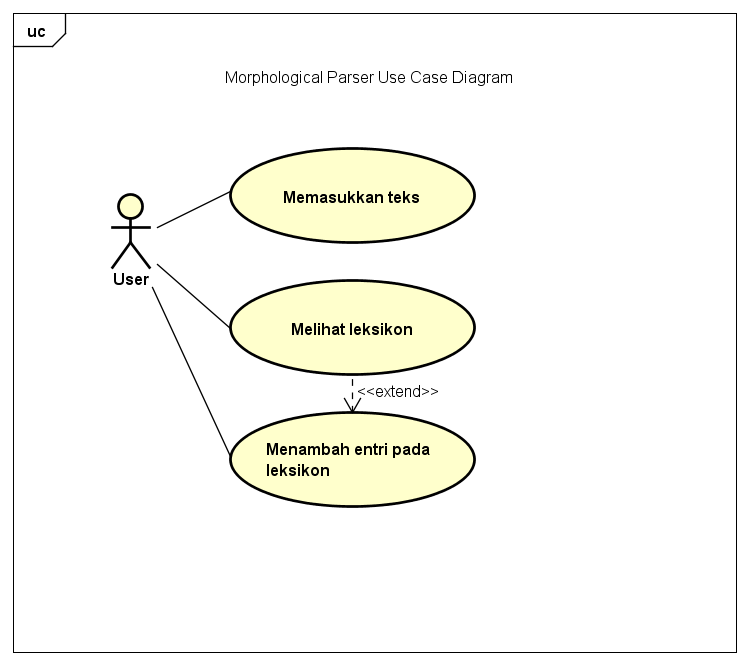
\includegraphics[scale=0.56]{Gambar/gambar-diagram-use-case}
\caption[Diagram use case perangkat lunak morphological parser]{Diagram use case perangkat lunak morphological parser} 
\label{gambar-diagram-use-case}
\end{figure}

Dari diagram tersebut dapat dituliskan use case scenario sebagai berikut:\\

\textbf{MEMPROSES TEKS}\\
\textbf{Name:} Memproses teks\\
\textbf{Actors:} User\\
\textbf{Goals:} User berhasil memproses teks melalui sistem\\
\textbf{Precondition:} Teks sudah disiapkan\\
\textbf{Steps:}

\begin{table}[H]
\centering
\begin{tabular}{|c|c|}
\hline
\textbf{Actor actions} & \textbf{System responses} \\
\hline
1. User memilih pilihan untuk& \\memasukkan teks melalui file&
2. Sistem menampilkan kotak dialog \\&untuk memilih file\\
3. User mengarahkan kotak dialog&\\ ke direktori tempat file teks masukan&\\
4. User menekan tombol "OK"&
5. Sistem menampilkan isi file \\&ke dalam kolom masukan\\
6. User menekan tombol "Proses"&7. Sistem menampilkan hasil proses\\&ke dalam kolom keluaran\\
\hline
\end{tabular}
\end{table}

\textbf{Alternate flow:}

\begin{table}[H]
\centering
\begin{tabular}{|c|c|}
\hline
\textbf{Actor actions} & \textbf{System responses} \\
\hline
1a. User menulis teks ke dalam kolom masukan&\\
2a. User menekan tombol "Proses"&3a. Sistem menampilkan hasil proses\\&ke dalam kolom keluaran\\
\hline
\end{tabular}
\end{table}

\textbf{MELIHAT ENTRI LEKSIKON}\\
\textbf{Name:} Melihat entri leksikon\\
\textbf{Actors:} User\\
\textbf{Goals:} User dapat melihat semua entri leksikon yang ada dalam sistem\\
\textbf{Precondition:} Sistem sudah memuat leksikon ke dalam program\\
\textbf{Steps:}

\begin{table}[H]
\centering
\begin{tabular}{|c|c|}
\hline
\textbf{Actor actions} & \textbf{System responses} \\
\hline
1. User memilih pilihan untuk&\\melihat leksikon&
2. Sistem menampilkan leksikon\\&yang ada dalam sistem \\
\hline
\end{tabular}
\end{table}

\textbf{MENAMBAH ENTRI PADA LEKSIKON}\\
\textbf{Name:} Menambah entri pada leksikon\\
\textbf{Actors:} Editor\\
\textbf{Goals:} Editor berhasil menambah entri pada leksikon\\
\textbf{Precondition:} Sistem sudah memuat leksikon ke dalam program\\
\textbf{Steps:}

\begin{table}[H]
\centering
\begin{tabular}{|c|c|}
\hline
\textbf{Actor actions} & \textbf{System responses} \\
\hline
1. Editor memilih pilihan untuk&\\ menambah entri pada leksikon&
2. Sistem menampilkan form untuk \\&menambah entri pada leksikon\\
3. Editor mengisikan entri baru pada form&\\
4. Editor menekan tombol "OK"&
5. Sistem mengeluarkan keterangan \\&"Entri berhasil dimasukkan"\\
\hline
\end{tabular}
\end{table}

\textbf{Alternate flow:}

\begin{table}[H]
\centering
\begin{tabular}{|c|c|}
\hline
\textbf{Actor actions} & \textbf{System responses} \\
\hline
&5a. Sistem mengeluarkan keterangan \\&"Format pengisian entri salah, ulangi lagi"\\
\hline
\end{tabular}
\end{table}

\textbf{MENGUBAH ENTRI PADA LEKSIKON}\\
\textbf{Name:} Mengubah entri pada leksikon\\
\textbf{Actors:} Editor\\
\textbf{Goals:} Editor berhasil mengubah entri pada leksikon\\
\textbf{Precondition:} Sistem sudah memuat leksikon ke dalam program\\
\textbf{Steps:}

\begin{table}[H]
\centering
\begin{tabular}{|c|c|}
\hline
\textbf{Actor actions} & \textbf{System responses} \\
\hline
1. Editor memilih entri leksikon yang akan diubah&\\
2. Editor memilih pilihan untuk&\\ mengubah entri pada leksikon&
3. Sistem menampilkan form untuk \\&mengubah entri pada leksikon\\
4. Editor melakukan perubahan entri pada form&\\
5. Editor menekan tombol "OK"&
6. Sistem mengeluarkan keterangan \\&"Entri berhasil diubah"\\
\hline
\end{tabular}
\end{table}

\textbf{Alternate flow:}

\begin{table}[H]
\centering
\begin{tabular}{|c|c|}
\hline
\textbf{Actor actions} & \textbf{System responses} \\
\hline
&6a. Sistem mengeluarkan keterangan \\&"Format pengisian entri salah, ulangi lagi"\\
\hline
\end{tabular}
\end{table}

\textbf{MENGHAPUS ENTRI PADA LEKSIKON}\\
\textbf{Name:} Menghapus entri pada leksikon\\
\textbf{Actors:} Editor\\
\textbf{Goals:} Editor berhasil menghapus entri pada leksikon\\
\textbf{Precondition:} Sistem sudah memuat leksikon ke dalam program\\
\textbf{Steps:}

\begin{table}[H]
\centering
\begin{tabular}{|c|c|}
\hline
\textbf{Actor actions} & \textbf{System responses} \\
\hline
1. Editor memilih entri leksikon yang akan dihapus&\\
2. Editor memilih pilihan untuk&\\ menghapus entri pada leksikon&
3. Sistem menampilkan kotak dialog \\&persetujuan menghapus entri\\
4. Editor menekan tombol "OK"&
5. Sistem mengeluarkan keterangan \\&"Entri berhasil dihapus"\\
\hline
\end{tabular}
\end{table}


\section{Diagram Kelas}
\label{sec:DiagramKelasAwal}

Berdasarkan analisis yang telah dilakukan, kelas-kelas yang akan dibuat untuk perangkat lunak morphological parser adalah sebagai berikut.

\textbf{Kelas Parser} berfungsi untuk melakukan proses parsing terhadap sebuah kalimat atau paragraf dalam bahasa Indonesia.

Atribut yang terdapat dalam kelas ini adalah:

\begin{itemize}
	\item \textit{parseResult}: bertipe String dan menyimpan hasil parsing dari kalimat atau paragraf yang menjadi masukan
	\item \textit{lexicon}: bertipe objek dari kelas Lexicon dan merupakan objek yang digunakan oleh kelas Parser untuk mengakses fitur leksikon dari perangkat lunak
\end{itemize}

Method yang terdapat dalam kelas ini adalah:

\begin{itemize}
	\item \textit{Parser}: konstruktor tanpa parameter untuk membuat objek dari kelas Parser.
	\item \textit{isRootWord}: method dengan sebuah parameter bertipe String dan kembalian bertipe boolean untuk menentukan apakah kata yang ada di parameter merupakan kata dasar atau bukan. Method ini memanggil method searchInTree dari kelas Lexicon.
	\item \textit{processFromText}: method dengan sebuah parameter bertipe String dan kembalian bertipe String untuk melakukan proses parsing terhadap teks yang ada di parameter.
	\item \textit{processFromFile}: method dengan sebuah parameter bertipe String dan kembalian bertipe String untuk melakukan proses parsing terhadap isi file dari path yang ada di parameter.
	\item \textit{checkPrefiks}: method dengan sebuah parameter bertipe String dan kembalian bertipe void untuk melakukan pengecekan ada atau tidak prefiks dalam String kata yang diberikan di parameter.
	\item \textit{checkSufiks}: method dengan sebuah parameter bertipe String dan kembalian bertipe void untuk melakukan pengecekan ada atau tidak sufiks dalam String kata yang diberikan di parameter.
	\item \textit{checkRedup}: method dengan sebuah parameter bertipe String dan kembalian bertipe void untuk melakukan pengecekan reduplikasi pada String kata yang diberikan di parameter.
	\item \textit{checkKonfiks}: method tanpa parameter dan kembalian bertipe void untuk melakukan pengecekan adanya kemungkinan kombinasi prefiks dan sufiks yang membentuk konfiks pada atribut hasil parsing.
	\item \textit{checkKomposisi}: method dengan sebuah parameter bertipe String dan kembalian bertipe void untuk melakukan pengecekan komposisi pada String kata yang diberikan di parameter.
	\item \textit{checkKomposisi}: method dengan sebuah parameter bertipe String dan kembalian bertipe void untuk melakukan pengecekan kemungkinan komposisi antara kata yang sedang diproses dengan String kata yang diberikan di parameter.
\end{itemize}

\textbf{Kelas Lexicon} berfungsi untuk menyimpan kumpulan kata dasar dan kata turunan yang digunakan selama proses morphological parsing berlangsung.

Atribut yang terdapat dalam kelas ini adalah:

\begin{itemize}
	\item \textit{roots}: bertipe array of Node dan menyimpan kumpulan akar dari pohon node yang menyimpan kata dasar yang valid dalam bahasa Indonesia
	\item \textit{components}: bertipe array of String dan menyimpan kumpulan kata turunan untuk setiap kata dasar dalam bahasa Indonesia
\end{itemize}

Method yang terdapat dalam kelas ini adalah:

\begin{itemize}
	\item \textit{Lexicon}: konstruktor tanpa parameter untuk membuat objek dari kelas Lexicon.
	\item \textit{insertRoot}: method dengan sebuah parameter bertipe String dan kembalian bertipe void untuk memasukkan sebuah kata dasar baru ke dalam leksikon.
	\item \textit{updateRoot}: method dengan dua buah parameter bertipe String dan kembalian bertipe void untuk mengubah kata dasar lama dalam parameter menjadi kata dasar baru dalam parameter.
	\item \textit{deleteRoot}: method dengan sebuah parameter bertipe String dan kembalian bertipe void untuk menghapus sebuah kata dasar dalam parameter.
	\item \textit{insertComponent}: method dengan dua buah parameter bertipe String dan kembalian bertipe void untuk memasukkan sebuah kata turunan baru dalam parameter ke kata dasar dalam parameter.
	\item \textit{updateComponent}: method dengan tiga buah parameter bertipe String dan kembalian bertipe void untuk mengubah kata turunan lama dalam parameter menjadi kata turunan baru dalam parameter untuk kata dasar dalam parameter.
	\item \textit{deleteComponent}: method dengan dua buah parameter bertipe String dan kembalian bertipe void untuk menghapus sebuah kata turunan dalam parameter dari kata dasar dalam parameter.
	\item \textit{searchInTree}: method dengan sebuah parameter bertipe String dan kembalian bertipe boolean untuk mencari kata dasar di parameter dalam pohon Node.
	\item \textit{printAllWordInTree}: method tanpa parameter dan kembalian bertipe String untuk mencetak semua kata yang disimpan dalam pohon Node ke dalam sebuah String.
\end{itemize}

\textbf{Kelas Node} berfungsi untuk menyimpan satu karakter dalam pohon Node.

Atribut yang terdapat dalam kelas ini adalah:

\begin{itemize}
	\item \textit{letter}: bertipe char dan menyimpan sebuah karakter
	\item \textit{endOfWord}: bertipe boolean dan menyimpan keterangan apakah node ini merupakan karakter akhir dari sebuah kata dalam pohon atau tidak
	\item \textit{children}: bertipe array of Node dan menyimpan kumpulan node yang merupakan anak dari node ini
	\item \textit{parent}: bertipe node dan menyimpan sebuah node yang merupakan parent dari node ini
\end{itemize}

Method yang terdapat dalam kelas ini adalah:

\begin{itemize}
	\item \textit{Node}: konstruktor tanpa parameter untuk membuat objek dari kelas Node.
\end{itemize}

Gambar \ref{gambar-diagram-kelas-awal} berikut adalah diagram kelas awal yang dibuat untuk perangkat lunak ini.

\begin{figure}[H]
\centering
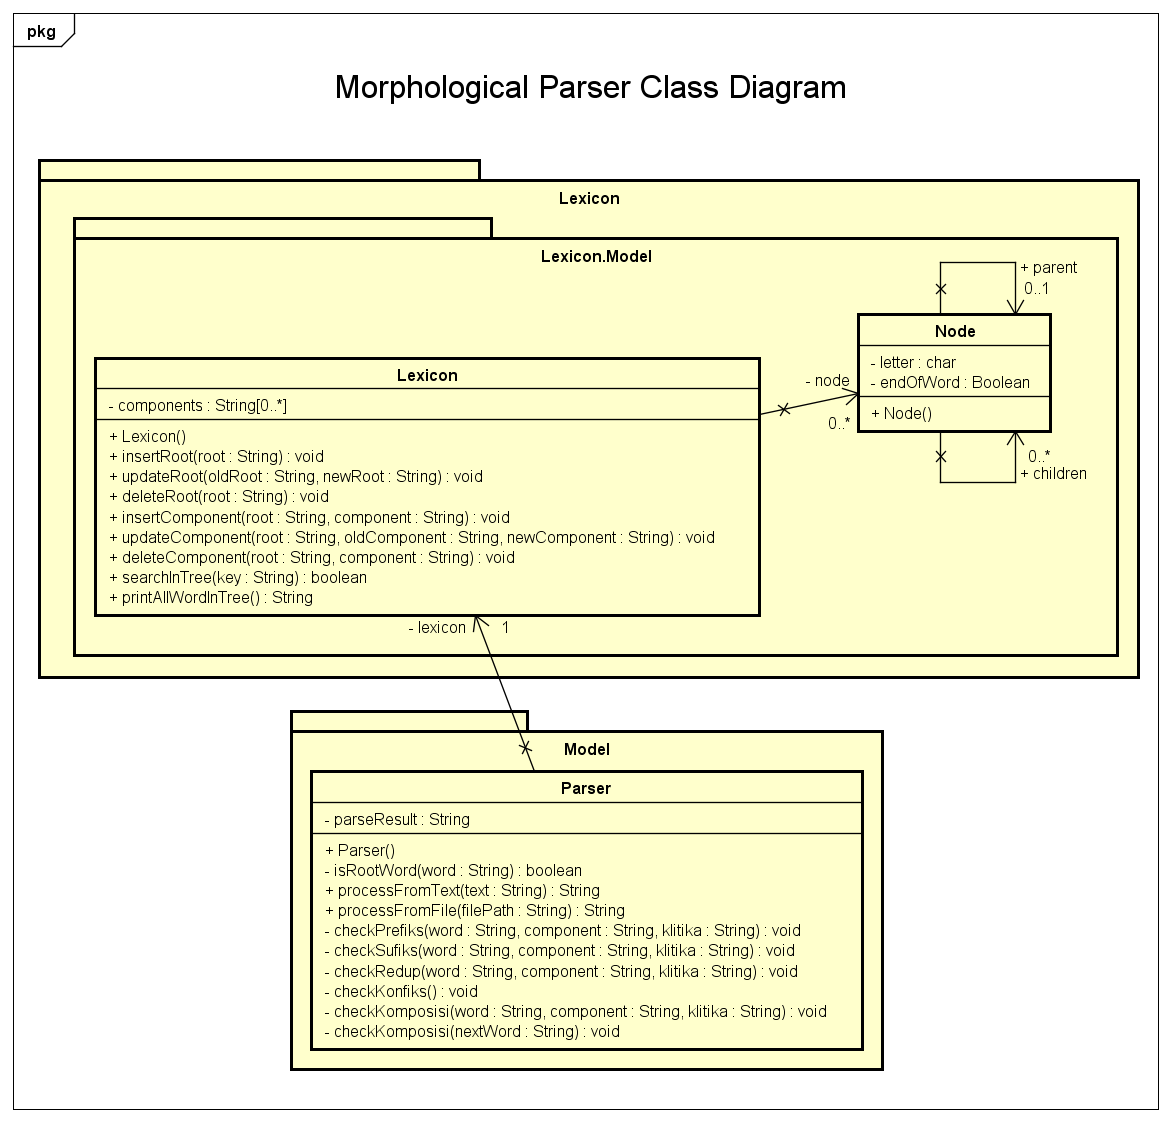
\includegraphics[scale=0.4]{Gambar/gambar-diagram-kelas-awal}
\caption{Diagram kelas awal perangkat lunak morphological parser} 
\label{gambar-diagram-kelas-awal}
\end{figure}